\documentclass[11pt,a4paper]{article}
\usepackage[T1]{fontenc}
\usepackage[margin=1in]{geometry}
\usepackage{amsmath,amssymb,mathtools}
\usepackage{booktabs}
\usepackage{graphicx}
\usepackage{xcolor}
\usepackage[colorlinks=true,linkcolor=blue!60!black,citecolor=blue!60!black,urlcolor=blue!60!black]{hyperref}
\usepackage{microtype}
\usepackage{enumitem}
\usepackage[most]{tcolorbox}
\usepackage{listings}
\lstset{basicstyle=\ttfamily\scriptsize,breaklines=true,columns=fullflexible,keepspaces=true,frame=single,framerule=0.3pt,xleftmargin=4pt}
\newcommand{\SpNumpyA}{4.3}
\newcommand{\SpBestA}{3.2}
\newcommand{\RustMsA}{0.62}
\newcommand{\NumpyMsA}{2.63}
\newcommand{\SpNumpyB}{4.2}
\newcommand{\SpBestB}{2.1}
\newcommand{\RustMsB}{2.73}
\newcommand{\NumpyMsB}{11.50}
\newcommand{\SpNumpyC}{2.7}
\newcommand{\SpBestC}{1.6}
\newcommand{\RustMsC}{22.52}
\newcommand{\NumpyMsC}{60.22}
\newcommand{\SpNumpyD}{2.5}
\newcommand{\SpBestD}{1.5}
\newcommand{\RustMsD}{104.60}
\newcommand{\NumpyMsD}{260.00}
\newcommand{\MaxChecksumDiff}{1e-13}
\newcommand{\CvodeOrder}{4.00}
\newcommand{\CvodeRhs}{482}
\newcommand{\CvodeSteps}{95}
\newcommand{\ThrRustOne}{300}
\newcommand{\ThrRustMax}{583}
\newcommand{\ThrNumpyOne}{42}
\newcommand{\ThrNumpyMax}{120}
\newcommand{\ThroughputRatio}{4.9}

\newcommand{\PENDING}[1]{\textcolor{red!70!black}{[pending: #1]}}
\newtcolorbox{keybox}[1][]{colback=blue!3,colframe=blue!45!black,boxrule=0.5pt,left=4pt,right=4pt,top=3pt,bottom=3pt,#1}
\newtcolorbox{failbox}[1][]{colback=red!3,colframe=red!45!black,boxrule=0.5pt,left=4pt,right=4pt,top=3pt,bottom=3pt,#1}

\title{\textbf{qf-pgpe: a verified pure-Rust projected Gross--Pitaevskii engine for quantum-fluid experiments, with a Python extension}\\
\large The quantum-fluids module of rusty-SUNDIALS --- design, cross-language verification, performance, and what porting found}
\author{Xavier Callens\\ \small SocrateAI-Scientific-QuantumFluids and rusty-SUNDIALS\\
\small \url{https://github.com/xaviercallens/rusty-SUNDIALS}}
\date{October 2026}

\begin{document}
\maketitle

\begin{abstract}\noindent
Classical-field (projected Gross--Pitaevskii) simulations of two-dimensional Bose fluids are usually scripts: an FFT library, a time stepper and
analysis code whose correctness is checked, when at all, by a few conservation laws. We describe \texttt{qf-pgpe}, the quantum-fluids module of
the rusty-SUNDIALS numerical library: a pure-Rust integrating-factor RK4 engine for the projected equation on a periodic grid, a vortex
instrument (periodic theta-function imprint, sub-grid detection, tracking), the registered estimators of vortex friction and diffusion, a thermal-state
toolkit and a vortex--phonon scattering instrument, plus a Python extension that exposes them on numpy arrays. Every module is a port of a
Python original of an ongoing, pre-registered research programme and carries a numeric cross-check against it: estimators agree to $2\times10^{-14}$
on real vortex tracks, a $31$-run scattering matrix to $5\times10^{-11}$, measurements on a shared thermal field to $10^{-14}$; the engine is checked against
independent known answers and against rusty-SUNDIALS' own CVODE (global error falling as $\Delta t^{\CvodeOrder}$). The cross-checks found three defects,
one of them in the Python programme: its primary estimator of the mutual friction is biased low by vortex diffusion ($-8$ to $-22\,\%$), a flaw the
registered synthetic gate had not shown. On a single thread of a 2013 laptop CPU the engine is $\SpNumpyA\times$, $\SpNumpyB\times$, $\SpNumpyC\times$ and $\SpNumpyD\times$ faster per step than the
numpy engine at $N=64$, $128$, $256$, $512$ ($\SpBestA\times$--$\SpBestD\times$ against the fastest of the Python engines we tried, torch on CPU), and a drop-in replacement of the
Python stepper makes an end-to-end thermal-state measurement $5.3\times$ faster with identical results. We make no claim about GPU codes or other
published solvers, which we did not measure; intra-run threading, tried, did not help on this machine.
\end{abstract}

\section{Introduction}

Finite-temperature quantum-fluid physics in two dimensions --- the Berezinskii--Kosterlitz--Thouless transition, the friction on a quantized vortex, the screening
by thermal vortex pairs --- is routinely studied with the projected Gross--Pitaevskii equation (PGPE)~\cite{Davis2001,Blakie2008}: a microcanonical classical field
$i\partial_t\psi=P[-\tfrac12\nabla^2\psi+g|\psi|^2\psi]$ with a sharp momentum cutoff $P$ that makes the thermal cloud, the condensate and the vortices
dynamical. The numerical core is small (a 2D FFT pair and a Runge--Kutta stepper); what is large, and error-prone, is what sits on top of it: imprinting vortices on a torus,
finding and following them, reading transport coefficients out of the tracks, measuring temperature and normal density of a state.

This paper describes the module of the rusty-SUNDIALS library~\cite{Hindmarsh2005} (a Rust implementation of the SUNDIALS solver suite) that carries this stack, \texttt{qf-pgpe},
and records what we can and cannot say about it. Its design rule is that no module is accepted without a direct numeric comparison against the original it replaces, on
the same inputs. Our contributions are: (i) the engine and instruments (Section~\ref{sec:design}); (ii) a verification record that includes independent integration by the library's own CVODE and
cross-language comparisons with quantified differences (Section~\ref{sec:verification}); (iii) the three defects this found (Section~\ref{sec:found}); (iv) measured performance against numpy, scipy and torch, with the conditions stated
(Section~\ref{sec:performance}); (v) a Python extension with a drop-in stepper (Section~\ref{sec:extension}). The physics results that the programme obtained with these tools are
published separately~\cite{Callens2026a,Callens2026b,Callens2026sw}; here they serve as use cases (Section~\ref{sec:use}).

\begin{keybox}
\textbf{What is claimed, and what is not.} Claimed: agreement with the Python originals at the stated levels; single-thread speed-ups over the numpy, scipy and torch-CPU engines on the
stated machine; bit-identical results between optimisations. \textbf{Not claimed:} that this is the best PGPE solver. We did not benchmark GPU codes, FFTW-based C codes or other published
solvers (none were installed), the machine is a 2013 quad-core laptop CPU, and the one parallelisation we tried inside a run gave no speed-up.
\end{keybox}

\section{Design}\label{sec:design}

\paragraph{Engine.} \texttt{ComplexField2D} integrates the projected equation on an $N\times N$ periodic grid of side $L$ ($\hbar=m=1$, interaction $g$) by the integrating-factor RK4 scheme: the linear
part is exact in Fourier space, the cubic part is classical RK4, the projector is a sharp circle $|k|\le k_{\rm cut}=f\,k_{\max}$ (default $f=1/2$, the cutoff at which the cubic term is alias-free in the interior of the retained set).
FFT conventions are numpy's (\texttt{fftfreq} ordering; unnormalised forward transform), so arrays are exchanged with the Python programme without conversion. Norm, energy and momentum are provided;
\texttt{rhs}/\texttt{pack}/\texttt{unpack} expose the right-hand side as an ODE system for external integrators.

\paragraph{Instruments.} Table~\ref{tab:modules} lists the modules. All are ports of the Python programme's scripts, with the same formulas and the same registered conventions.

\begin{table}[h]\centering\small
\begin{tabular}{p{0.14\linewidth}p{0.5\linewidth}p{0.26\linewidth}}\toprule
module & content & Python original\\\midrule
\texttt{lib} & IF-RK4 PGPE, cutoff fraction, invariants, \texttt{rhs}/\texttt{pack}/\texttt{unpack} & \texttt{pgpe.py}\\
\texttt{vortex} & periodic theta-function imprint with Bernoulli amplitude, raw plaquette detection with sub-grid refinement, tracker, tracked runs, placements & \texttt{vortex\_transport.py}\\
\texttt{transport} & estimators of $\alpha$ (energy, regression), $1-\alpha'$, $\eta$ (residual MSD), block jackknife; point-vortex velocity/energy on the torus; synthetic Langevin gate G0 & \texttt{transport\_estimators.py}\\
\texttt{thermal} & seeded RNG, \texttt{random\_state}, \texttt{heat}, thermometer, condensate fraction, current correlators ($n_s/n$), vortex count, Fourier resampling, \texttt{run\_blocks}, \texttt{make\_base} & \texttt{observables.py}, \texttt{round2.py}\\
\texttt{scattering} & Bogoliubov-wave dressing of a vortex pair, wave momentum flux, drift slopes, $\sigma_\parallel(k)$, $\sigma_\perp(k)$; parallel resumable scan runner & \texttt{vortex\_wave\_scattering.py}\\
\texttt{qf-pgpe-py} & Python extension (pyo3, numpy) & ---\\\bottomrule
\end{tabular}
\caption{The modules of the quantum-fluids crate. Not ported (declared): the $g_1$ correlation fits, vortex--dipole matching, the Onsager order parameter, persistent-homology instruments and the symbolic series of the programme.}\label{tab:modules}
\end{table}

\paragraph{Performance engineering.} The step is allocation-free (a workspace is allocated once per run, two ping-pong buffers carry the state) and the 2D FFT is rows--transpose--rows with a tiled in-place transpose (unit stride in both passes). In the nonlinear term the
FFT lines that are identically zero in a projected field (rows with no mode inside the projector on the way in) or are discarded by the projector (on the way out) are not transformed; this is exact (a test asserts equality bit for bit for three cutoffs) and gave $8$--$11\,\%$.
A rayon-parallel pass over rows was implemented and removed: on this four-core machine it gave no speed-up at $N=512$ and $1024$ with two and four threads, and independent runs --- the unit in which the programme parallelises --- scale across processes (Section~\ref{sec:performance}).

\section{Verification}\label{sec:verification}

\paragraph{Known answers.} The engine carries the programme's pre-registered known answers: norm conservation ($10^{-8}$), momentum conservation ($10^{-10}$ for states with weight away from the cutoff edge), the exact plane-wave solution ($10^{-9}$),
and, for the vortex instrument, the $T=0$ gate of the campaign (a neutral pair neither shrinks nor changes momentum; momentum $0.96$--$0.99$ of $2\pi nd$; exactly two detections).

\paragraph{An independent integrator: CVODE.} The right-hand side of the projected equation, on the retained modes, is an ODE system of dimension $2N_{\rm modes}$. We hand it, unchanged, to rusty-SUNDIALS' variable-order Adams solver with tight tolerances
($N=16$, $L=16$, $49$ modes, $t=1$) and use the result as an independent reference. The global error of the IF-RK4 step falls as $\Delta t^{\CvodeOrder}$ over $\Delta t=0.04\ldots0.0025$ (Fig.~\ref{fig:verif}, left), which is the order the programme registered (its ``K2'' check, previously not ported).
The test depends on a fix of the library (the Adams order was stuck at one): without it the solver collapses its step on this oscillatory Hamiltonian problem and fails after about $10^6$ right-hand-side evaluations; with it, \CvodeRhs\ evaluations in \CvodeSteps\ steps. The test is therefore also a regression guard for the solver.

\begin{figure}[h]\centering
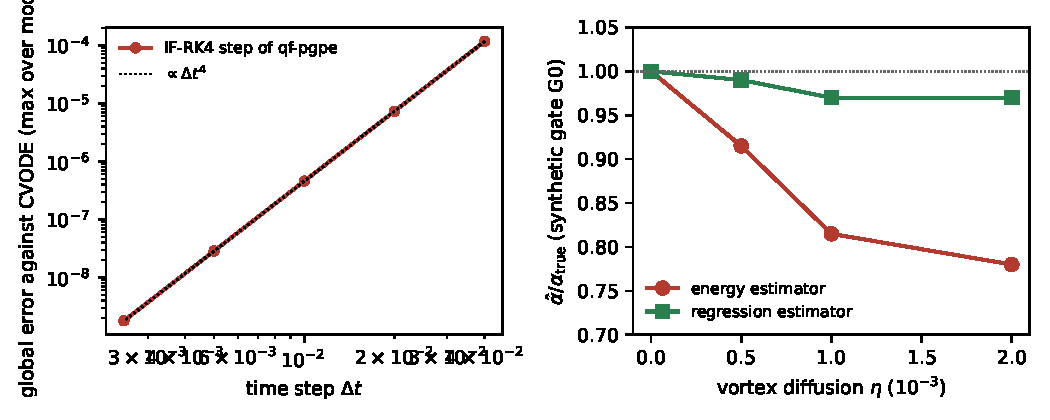
\includegraphics[width=\linewidth]{figures/sw_fig2_verification.pdf}
\caption{Left: global error of the IF-RK4 step against a CVODE reference of the same right-hand side. Right: the energy estimator of the friction is biased low by diffusion in the registered synthetic gate (a flaw found by the port, Section~\ref{sec:found}).}\label{fig:verif}
\end{figure}

\paragraph{Cross-language agreement.} Table~\ref{tab:cross} gives the measured differences between each Rust module and its Python original on the same inputs.

\begin{table}[h]\centering\small
\begin{tabular}{p{0.2\linewidth}p{0.48\linewidth}p{0.22\linewidth}}\toprule
module & comparison (same inputs) & max difference\\\midrule
transport & four real vortex tracks (800 samples), every estimate and error, non-default options & $2\times10^{-14}$ relative (two estimators bit-identical)\\
thermal & one shared thermal field ($N=32$): norm, energy, $T$ (two windows), condensate fraction, $J_L$, $J_T$, vortex count & $\le3\times10^{-14}$; count exact\\
thermal & the same field after $20$ time units & $2.7\times10^{-12}$\\
scattering & short case, three runs: positions, momentum, energy, slopes & $7\times10^{-14}$, $8\times10^{-13}$, $3\times10^{-14}$\\
scattering & full probe ($L=64$, $N=128$, $400$ time units): $\sigma_\parallel$, $\sigma_\perp$ & identical to six digits ($2.03913$, $1.58133$)\\
scattering & the registered matrix ($31$ runs, $15$ points) & $4.6\times10^{-11}$ relative\\
vortex & imprint at positions with a vortex on a grid node; $T=0$ separation at $t=5$, $40$ ($N=64$) & $10^{-4}$ (after a defect fix)\\
extension & \texttt{run} $20$ time units ($N=64$); \texttt{imprint\_v2}; \texttt{detect}; \texttt{analyse\_tracks} & $10^{-10}$; $10^{-11}$; identical; bit-identical\\\bottomrule
\end{tabular}
\caption{Rust against Python on identical inputs. The random-number generators differ (xoshiro256** against numpy's PCG64), so constructions that draw random numbers (\texttt{random\_state}, \texttt{heat}) are compared statistically, measurements on a given field exactly.}\label{tab:cross}
\end{table}

\paragraph{A statistical comparison that did not meet its criterion.} For the thermal-state constructor ($N=64$, $L=32$, $e=0.6$, nine seeds each) the temperatures are $0.0757$ (Rust) and $0.0865$ (Python), per-seed standard deviations $0.018$ and $0.010$: a $12.5\,\%$ gap at $z=-1.6$, outside the $10\,\%$ criterion first set and not significant; a $60$-seed comparison at another configuration cannot distinguish the two
(vortex count $0.67$ against $0.57$, condensate fraction $0.739\pm0.009$ against $0.727\pm0.014$). The test asserts $|z|<2.5$; we report the gap rather than the criterion.

\paragraph{Platform dependence.} The scattering cross-check passes at $10^{-13}$ on x86-64 Linux, where its numpy fixtures were made, but its $T=0$ control run differed by $8\times10^{-3}$ in position on an Apple-silicon CI runner: a pair near the unstable saddle at $d=L/2$ amplifies rounding differences between libm and FFT kernels. The tolerances are strict on the reference platform and relaxed elsewhere.

\section{What porting found}\label{sec:found}

\begin{enumerate}[nosep]
\item \textbf{A defect in the first Rust version}, found by the vortex cross-check: a vortex centred exactly on a grid node was imprinted with unit modulus instead of zero. Fixed; the separation now agrees to $10^{-4}$.
\item \textbf{A bias in the Python programme's friction estimator.} The port of the estimators was bit-identical to Python on real tracks; running the registered synthetic gate over many seeds then showed that the energy estimator of $\alpha$ is biased low by vortex diffusion: for a true $\alpha=0.02$ it returns $0.0200$ at $\eta=0$ and $0.0183$, $0.0163$, $0.0156$ at $\eta=5\times10^{-4}$, $10^{-3}$, $2\times10^{-3}$ ($-8$, $-18$, $-22\,\%$), independently of the detection noise, while the regression estimator is unbiased
(Fig.~\ref{fig:verif}, right). The registered gate had passed on a single seed (its criterion passes on $2$ of $12$). The programme's published friction values were corrected~\cite{Callens2026a,Callens2026b}.
\item \textbf{A hidden dependency of the solver library}: the Adams-order defect above, exposed by the first Hamiltonian system run through CVODE.
\end{enumerate}

\section{Performance}\label{sec:performance}

\paragraph{Method.} The problem is identical in every engine: $N\times N$ grid, $L=N/2$, $g=1$, $\Delta t=0.01$, cutoff $k_{\max}/2$, one fixed initial state; the final states of all engines agree to \MaxChecksumDiff\ (relative difference of the checksum $\sum|{\rm Re}\,c|+|{\rm Im}\,c|$), so the timings are for the same computation.
Engines: numpy (pocketfft)~\cite{Harris2020}, scipy.fft with one and four workers~\cite{Virtanen2020}, torch on CPU with one and four threads~\cite{Paszke2019}, and \texttt{qf-pgpe} on one thread. Statistic: the best of the repetitions (three and five, in two measurement sessions) of the time per step, taken for every engine in the same way.
\textbf{Machine and conditions:} Intel Core i7-4930MX (2013, 4 cores/8 threads, AVX), Linux, no GPU; during the measurement an unrelated four-thread training job of another project was running, so absolute times are pessimistic and the best-of statistic is used for all engines alike. JAX could not be imported in this environment, FFTW-based C codes and GPU codes were not available: \textbf{no comparison with them is made}.

\begin{figure}[h]\centering
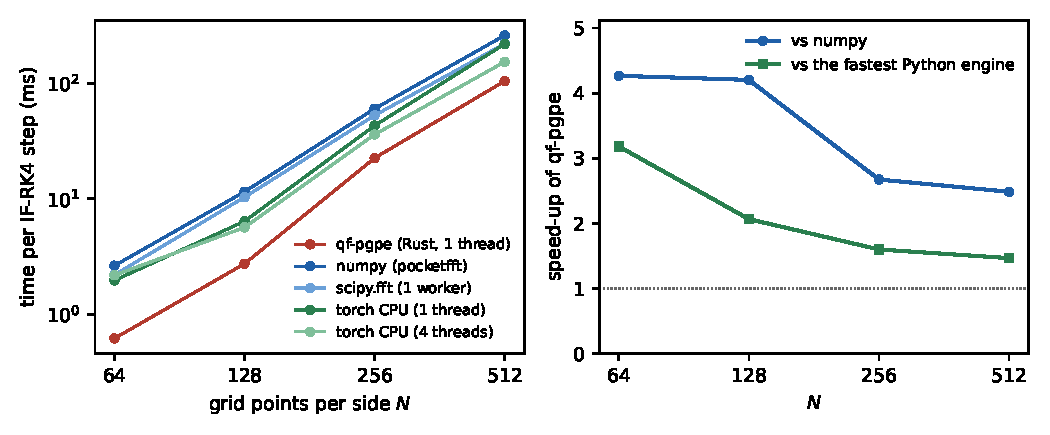
\includegraphics[width=\linewidth]{figures/sw_fig1_performance.pdf}
\caption{Time per IF-RK4 step against grid size for the engines of the benchmark (left) and the speed-up of \texttt{qf-pgpe} on one thread (right).}\label{fig:perf}
\end{figure}

\paragraph{Results.} On one thread \texttt{qf-pgpe} takes \RustMsA, \RustMsB, \RustMsC\ and \RustMsD\,ms per step at $N=64$, $128$, $256$, $512$, against \NumpyMsA, \NumpyMsB, \NumpyMsC\ and \NumpyMsD\,ms for numpy: speed-ups of \SpNumpyA, \SpNumpyB, \SpNumpyC\ and \SpNumpyD. Against the fastest Python engine at each size (torch on CPU, which is multi-threaded in its four-thread form)
the speed-up is \SpBestA, \SpBestB, \SpBestC\ and \SpBestD. The advantage shrinks with $N$. We did not profile the origin of the advantage; the step is dominated by FFTs, and the optimisations we measured separately (allocation-free loop, unit-stride transforms, pruned transforms) are each of the order of ten to seventy per cent.

\begin{figure}[h]\centering
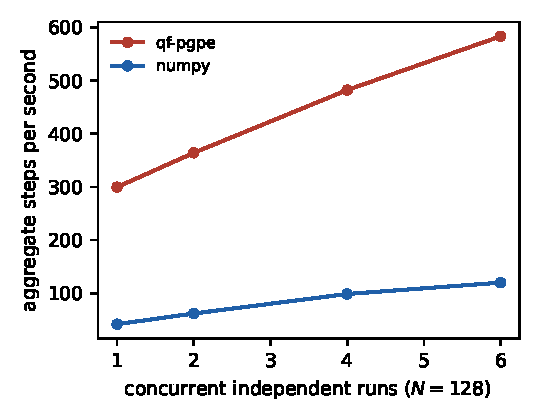
\includegraphics[width=0.55\linewidth]{figures/sw_fig3_throughput.pdf}
\caption{Aggregate throughput of independent runs ($N=128$, one thread each) against the number of concurrent processes, on the same machine and under the same external load.}\label{fig:thr}
\end{figure}

\paragraph{Throughput and end-to-end use.} The programme's experiments are many independent runs (seeds, pair sizes, wavenumbers), so throughput is the relevant quantity: with no interpreter lock and no per-step round trip, one process delivers \ThrRustOne\ steps per second at $N=128$ (numpy: \ThrNumpyOne) and the best aggregate over the concurrency we tried is \ThrRustMax\ against \ThrNumpyMax, a ratio of \ThroughputRatio\ (Fig.~\ref{fig:thr}).
End to end: a $50$-time-unit tracked $T=0$ vortex run at $128^2$ takes $41$\,s of CPU in Rust against $106$\,s in numpy ($2.6\times$), and a thermal-state measurement (\texttt{run\_blocks}, $60$ time units with measurements, $N=64$) takes $20.8$\,s with the drop-in extension against $109.8$\,s ($5.3\times$) with the same $T$, $n_s/n$, vortex count and energy (the measurement code is the same Python).

\section{The Python extension}\label{sec:extension}

The extension \texttt{qf\_pgpe} (pyo3 and the numpy crate) exposes \texttt{Pgpe} (\texttt{run}, \texttt{step}, invariants, \texttt{imprint\_v2}, \texttt{detect}, \texttt{momentum\_band}) and \texttt{analyse\_tracks} on C-contiguous \texttt{complex128} arrays of the numpy layout; \texttt{run} evolves for a given time inside one call with the interpreter lock released.
A subclass of the programme's Python stepper replaces only the stepping:

\begin{lstlisting}[language=Python]
from pgpe_rust import PGPERust as PGPE      # every script that did `from pgpe import PGPE` now steps in Rust
s = PGPE(N=128, L=64.0); c = s.run(c, 100.0) # callbacks keep their contract (chunked evolution)
\end{lstlisting}

so the measurement code is unchanged. A smoke test (the exact plane wave, conservation, imprint and detection, input validation) accompanies the crate.

\section{Use in the research programme}\label{sec:use}

The tools have been used in a pre-registered programme whose results are published separately: the vortex-transport paper~\cite{Callens2026a} (friction, diffusion and screening of vortices in a closed field), the friction-law paper~\cite{Callens2026b} (the friction follows the temperature, not the normal density), and the software record~\cite{Callens2026sw}. Two uses are specific to this module. First, the $31$-run vortex--phonon scattering matrix was reproduced independently in Rust, point by point, to $5\times10^{-11}$; the follow-up with a larger box (amendment WS-A2) and the replication of the pair-separation matrix are run on it. Second, the estimator bias of Section~\ref{sec:found} would not have been found by re-running the same code: it needed a second implementation and a seed sweep that was cheap enough to run.

\section{Limitations and future work}

\begin{itemize}[nosep]
\item One machine, one CPU generation, a concurrent external load; no GPU and no comparison with other published solvers. A GPU backend and a comparison with FFTW-based C codes are the obvious next measurements.
\item Intra-run parallelism did not help here (cause not investigated); large single simulations on many cores are not served.
\item The thermal constructors use their own RNG; reproducing a numpy-seeded construction bit for bit is not possible and not a goal.
\item The module is two-dimensional and periodic; the programme's three-dimensional and trapped geometries are not covered.
\item Momentum is conserved to $\sim10^{-6}$ (not $10^{-10}$) for noisy fields with weight at the cutoff edge, where the cubic term aliases; the numpy engine shows the identical drift.
\end{itemize}

\section{Availability}

Source: \url{https://github.com/xaviercallens/rusty-SUNDIALS} (crates \texttt{qf-pgpe}, \texttt{qf-pgpe-py}; pull request \PENDING{PR number once merged}); BSD-3-Clause. The Python programme, the benchmark script (\texttt{exploration/pgpe/bench\_engines.py}), the data (\texttt{data/generated/pgpe/bench/}) and the ledger are in~\cite{Callens2026sw}. Reproduction: \texttt{cargo test --release -p qf-pgpe} (27 tests), \texttt{python3 exploration/pgpe/bench\_engines.py single}.

\bibliographystyle{unsrt}
\bibliography{refs_software,refs_vortex_transport}
\end{document}
